\begin{frame}[fragile]{Nearest neighbor data structures for arbitrary metric spaces}

%\begin{tikzpicture}
%\node at (0,2) {
    %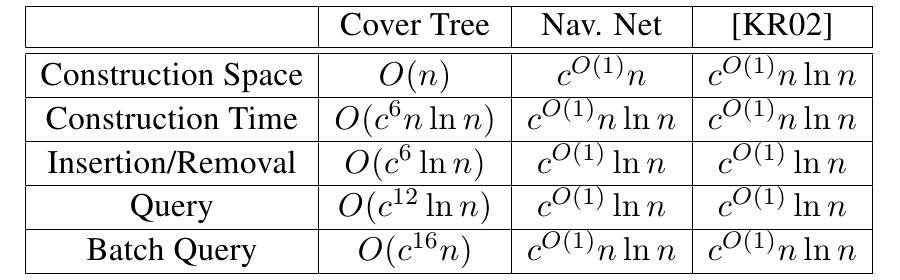
\includegraphics[width=12cm]{covertree/runtimes}


{\footnotesize
    \begin{tabular}{>\centering m{2cm}|>\centering m{2.0cm}|>\centering m{2.0cm}|>\centering m{2.0cm}|c}
    \hline
    & \footnotesize Cover Tree
    & \footnotesize Nav. Net
    & \footnotesize Met. Skip List
    & \footnotesize Ball Tree
    \\
    \hline
    \hline
    Construction space & $O(n)$ & $c^{O(1)}n$ & $c^{O(1)}n \log n$ & $O(n)$ \\
    Construction time & $O(c^6 n\log n)$ & $c^{O(1)}n\log n$ & $c^{O(1)}n \log n$ & $O(n^2)$ \\
    Insertion time (1 pt) & $O(c^6 \log n)$ & $c^{O(1)}\log n$ & $c^{O(1)} \log n$ & $O(n)$ \\
    Query time ~~~(1 pt) & $O(c^{12} \log n)$ & $c^{O(1)}\log n$ & $c^{O(1)} \log n$ &  $O(n)$\\
    Query time ~~~(n pts) & $O(c^{16} n)$ & $c^{O(1)}n\log n$ & $c^{O(1)}n \log n$ &  $O(n^2)$\\
    \hline
    & \footnotesize Beygelzimer ~~~\emph{et. al.}, 2006
    & \footnotesize Krauthgamer and Lee, 2004
    & \footnotesize Karger and Ruhl, 2002
    & \begin{tabular}{c}
        Omohundro,\\
        1989
      \end{tabular}
    \\
    \hline

    \end{tabular}
}
%};

\vspace{0.05in}
The variable $c$ is a measure of dimension (defined on next slide).

%\footnotesize
%\node at (-1,-0.4) { (Beygelzimer \emph{et. al.}, 2006)};
%\node at (2,-1) { (Krauthgamer and Lee, 2004)};
%\node at (4,-0.4) { (Karger and Ruhl, 2002) };
%\draw[->] (-1,-0.25) -- (-0.9,0.1);
%\draw[->] (1.3,-0.75) -- (1.5,0.1);
%\end{tikzpicture}

%Karger and Ruhl, Symposium on the Theory of Computing, 2002
%
%\vspace{0.15in}
%Krauthgamer and Lee, Symposium on Discrete Algorithms, 2004
%
%\vspace{0.15in}
%Beygelzimer, Kakade, and Langford, ICML, 2006

\vspace{0.05in}
Recent research either:
\begin{itemize}
\item Extends the analysis on cover trees {\footnotesize (Ram \emph{et. al.}, 2010; Curtin \emph{et. al.}, 2013)}
\item Focuses on \emph{approximate} queries (too many papers to list)
\end{itemize}

%\vspace{0.15in}
%More recent research focuses on \emph{approximate} queries: LHS, Spill trees
%\textbf{open problem}: construct a data structure in time $O(c^{O(1)}n)$ for some dimensionality $c$; is it even possible?
%\vspace{0.15in}

\end{frame}

